\documentclass[a4paper,10pt]{article}
\usepackage[a4paper,margin=1in]{geometry}
\usepackage{fancyhdr}

\usepackage{graphicx}
\usepackage{epsfig}
    
% setup fancy header, footer, and page count
\pagestyle{fancy}
\usepackage{lastpage}
\lhead{B. P. Wise}
\rhead{Pragmatic Affinity}
\lfoot{\textbf{\color{red}{DRAFT}}}
\cfoot{}
\rfoot{Page \thepage\ of \pageref{LastPage}}

\usepackage{amsmath} 
\usepackage[utf8]{inputenc}
\usepackage{color}


%opening
\title{Pragmatic Affinity in KTAB}
\author{Ben P. Wise, KAPSARC, \textbf{\color{red}{DRAFT v04}}}



%\setlength{\parindent}{4em}
\setlength{\parskip}{1em}

\begin{document}

\maketitle
\thispagestyle{fancy}

\begin{abstract}


In the common models of bargaining and negotiation in the spatial model of politics, the actors have both
publicly advocated positions and privately held ideals.
The ideals are assumed to either remain constant, or to simply reflect the current advocated position.
This document adds two kinds of flexibility to this mode. First, an actor's  ideal is adjusted toward the
advocated positions by a fractional amount: it could be 0\%, 100\%, or any value in between.
Second, the ideal could be adjusted not only toward the actor's own advocated position, but also toward the 
advocated position of other actors. This could represent affinity based on personal mentorship, ethnic ties,
and so on.

\end{abstract}


\section{Notation}
In the standard KTAB notation, the position of actor $i$  at turn $t$ is denoted by $\theta_{it}$.
In the spatial model of politics (SMP), the position is a point in a one- or multi-dimensional space.
The most common one-dimensional example is the left-right political spectrum. It is sometimes refined
into a two-dimensional space, with one axis representing economic centralization or decentralization 
and the other
axis representing social conservativism to liberalism. 
The number of dimensions is $K$, and they are indexed by $k$.


\section{Unilateral Adjustment}

In the first standard model of SMP bargaining, the public positions $\theta_{it}$ vary over time
while the ideals remain fixed at their initial values. 
Because the symbol $p$ is used elsewhere in KTAB to denote probabilities, we will denote the ideal position of 
actor $i$  at turn $t$ is denoted by $q_{it}$.
We will call this model of unvarying ideals the ``idealistic'' model,
and it is expressed in symbols as follows:

\begin{equation}
q_{i,t} = q_{i,0}
\end{equation}


In the second standard model of SMP bargaining, the public positions $\theta_{it}$ vary over time
while the ideals change to whatever was most recently advocated. We will call this the ``cynical'' model,
and it is expressed in symbols as follows:

\begin{equation}
q_{i,t} = \theta_{i,t}
\end{equation}

In our proposed model of flexible adjustment, the ideals would move only a fraction of the way
toward the current positions. The fractional adjustment is specified by the parameter $a_i$, as follows.

\begin{equation}
 q_{i,t+1} =  a_i  \theta_{i,t+1}  + (1-a_i) q_{i,t}
\end{equation}

The idealistic model sets $a_i = 0$ for all actors, while the cynical model sets $a_i = 1$ for all actors.
We propose to allow $0 \le a_i \le 1$, where each actor could potentially have different adjustment rates.
We will call this the ``pragmatic'' model, which reflects the vagueness of the term: some degree of holding
to ideals, and some degree of adjusting to the situation.


\section{Multilateral Adjustment}

The second extension to the adjustment model is to respond not only to the actor's own position
but to the positions of other actors as well.

We denoted actor $i$'s rate of adjustment toward actor $j$'s position by $a_{ij}$. We now define the
parameter $a_i$ as the sum of the adjustment rates. Again, the parameters are bounded by zero and one: 

\begin{align}
   a_i   & = \sum_{j} a_{ij}\\
    0    & \le a_{ij}\\
   a_i   & \le 1
\end{align} 

The adjustment of ideals is now specified by a weighted mixture of the new positions, and the old ideal:

\begin{equation} \label{eq:accomodation}
 q_{i, t+1} = \sum_{j} { a_{ij} \theta_{j, t+1} }  + (1-a_i) q_{i, t}
\end{equation}

Note that if actor $i$ has  $a_{ii} = 1$, then all of its other $a_{ij}$ coefficients must be zero,
and it just resets its ideal to its new position. Similarly, if actor $i$ has all $a_{ij} = 0$, then $a_i$ is zero, and its ideal stays at its initial value. Finally, if each
actor $i$ has  $a_{ii} < 1$ and all of its other $a_{ij} = 0$, then its ideal points simply
lag behind its public positions. 

To reflect the mix of pragmatism and affinity for certain others' positions,
we call this the ``pragmatic affinity'' model.

\section{Utility Calculations}

In some common models of utility in the SMP, the utility to actor $i$ of the position advocated by actor $j$
depends quadratically on the distance between $i$'s ideal and $j$'s position. To avoid excessive subscripts, 
we will temporarily drop the $t$ subscript when it would be the same for all variables in an equation.
The precise shape of the quadratic is specified by a curvature factor $-1 \le R_i \le +1$ reflecting $i$'s 
risk attitude:


\begin{equation} \label{eq:util_from_dist}
 u_{ij}    = (1- d_{ij}) (1+R_i d_{ij})
\end{equation}

The weighted distance is actually a  weighted Euclidean distance, using $i$'s salience along each dimension:

\begin{equation}\label{eq:weighted_dist}
  d^2_{ij}    = \frac{\sum_{k} [s_{ik} (q_{ik} - \theta_{jk})]^2 }{\sum_{k} [s_{ik}]^2 }
\end{equation}

In the idealistic model, all $a_{ij} = 0$, so the actor always compares other's positions to their 
unchanging ideal: $q_{it} = q_{i0}$. In the cynical model, $a_{ii} = 1$, so the actor 
compares others' positions
to their own current position: $q_{it} = \theta_{it}$. 
  


The distance in equation (\ref{eq:util_from_dist}) must be between zero and one. To ensure
this, not only is each
axis  limited to the $[0,1]$ range, so $ 0 \le | q_{ik} - \theta_{jk}| \le 1$, but also 
equation (\ref{eq:weighted_dist})  has a normalization
factor in the denominator.

Each individual salience must  be non-negative, at least one dimension must have positive salience,
and the total salience cannot be more than one:

\begin{align}\label{eq:salience} 
  0          & \le s_{ik} \\
  s_i        & = \sum_{k} s_{ik} \\
  0          & < s_i \\
  s_i        & \le  1
\end{align}
  
  
\section{Consequences for Bargaining}

Letting ideals differ from positions fundamentally changes the dynamics of a model,
as we will illustrate for the spatial model of policits.
When ideals always adjust 100\% to the current position, the actors
 always prefer their current position over any other. Thus, if actor $i$ would like
for actor $j$ to change their position, it would never be in $j$'s perceived self-interest
to do so.

\begin{figure}[h]
  \centering
  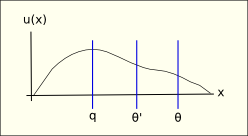
\includegraphics{./welcome-change.png}
  \caption{Desirable Change in Position}
  \label{fig:welcom-pos-change}
\end{figure}




However, if ideals can differ from positions, then situations can arise such as
figure (\ref{fig:welcom-pos-change}). In this situation, actor $j$'s utility
is peaked at their ideal, which  is the left-most point, $q$. Its current position
is the right-most point, $\theta$. Now suppose actor $i$ proposes that $j$ adopt
a new position, $\theta'$, more to $i$'s liking than $\theta$.
In this case, $j$ would not resist the change but would
actually support $i$'s proposed bargain.

Mathematics aside, it is easy to see   how this could happen in practice. Suppose $j$
has been led by external circumstances to adopt a policy position different from their ideal.
In other words, the current position was the best they thoght they could plausibly
pursue, but 
they would really rather, in an better situation, pursue a  policy closer to their true ideals
- if only there were sufficient support to make it feasible.
When $i$ proposes that $j$ adopt a policy more in line with $i$'s preferences,
this could be greeted with relief rather than resistance, because
it gives $j$ the support to drop pretenses, compromise less,  and pursue a less hypocritical policy.


\section{Sequencing}
The KTAB system is a toolkit for building models, so there are many ways to construct bargaining
models in KTAB that implement some version of the spatial model of politics. The difference is 
which particular algorithm they use for bargaining;
the pragmatic affinity sub-model is consistent with many of them. In KTAB,
the collective decision making process always proceeds by a series of turns, until some stopping
criterion is met. The initial state is always designated as time 0.

Suppose a turn starts at time $t$. The actors already have positions and ideals $\theta_{it}$
and $q_{it}$, respectively. The particular bargaining algorithm used will 
determine some set of new positions, $\theta_{i,t+1}$,
 based on the current  $\theta_{it}$
and $q_{it}$. These will be the advocated postions in the new state at time $t+1$.
Next, there is an ``accomodation'' phase, wherein all the new ideals are determined
according to equation (\ref{eq:accomodation}). This determines the ideals $q_{i,t+1}$ for the new state,
and the cycle is then ready to repeat for the next turn.

  
\section{Extensions}

The idea of evaluating the attractiveness of a policy by its effect on affinity groups can be extended to
non-SMP models in KTAB. For example, the standard distribution of KTAB includes several example programs
to illustrate how to build both SMP and non-SMP model. 
One example is \mbox{\texttt{leonApp}}, which  uses a simple Leontief input/output 
model to assess the economic consequences of revenue-neutral tax and subsidy policies.
Currently, the actors look only at the economic effects on themselves, though they may modify their positions
to win support from others, thus increasing the likelihood of an outcome favorable to themselves.

The pragmatic affinity approach could be extended to this by having the actors look not only at the economic 
effect upon themselves, but also on the effect upon various friends and enemies. For example, an actor
who forms economic policy with an eye toward their patronage network might heavily weight the benefit
to those actors from whom they expected to receive patronage (up),
or whose loyalty they need to maintain (down).

This would result in actors negotiating not just bargains which are likely to benefit
themselves, but also bargains which are likely to benefit their patronage network, either up or down.
 
\end{document}
